\documentclass[11pt]{article}

\usepackage[ngerman]{babel}
\usepackage[T1]{fontenc}
\usepackage[utf8]{inputenc} 
\usepackage[pdftex]{graphicx}
\usepackage{pdfpages}
\usepackage{geometry,blindtext}

\geometry{a4paper,left=30mm,right=20mm, top=1cm, bottom=2cm, includeheadfoot}

\usepackage{float}

\usepackage{amsmath, amsthm, amssymb}

\usepackage[babel,german=quotes]{csquotes}


\usepackage{fancyhdr}
\pagestyle{fancy}
\fancyhf{}

\fancyfoot[L]{\small{\textbf{Basistechniken\\Miniprojekt Auslandssemester}}}

\fancyhead[L]{\small{David Brüggemann, Patrick Kotz, Merlin Fischer}}

\fancyhead[R]{\today}

%\renewcommand{\headrulewidth}{0.5pt}

% Bei Problemen mit Umlauten:
% "uft8" durch "latin1", "ansinew" oder "applemac" ersetzen.

\begin{document}


\begin{titlepage}
  \title{Projektmanagment: \\Auslandssemester in Windhoek, Namibia}
  \author{Patrick Kotz, David Brüggemann, Merlin Fischer,\\ Fachhochschule Südwestfalen}
  \date{\today}
\end{titlepage}

\fancyfoot[C]{\thepage}

\maketitle

\newpage
\tableofcontents
\newpage

\section{Einleitung}
Ein Auslandsstudium bezeichnet einen Studienaufenthalt von meist ein bis zwei Semestern in einem anderen Land als dem, in dem das Studium aufgenommen wurde und normalerweise auch abgeschlossen werden kann.

\section{Projektauftrag}
Wir wollen ein Auslandssemester in der Universität Polytechnic of Namibia in Windhoek erfolgreich absolvieren und ohne große finanzielle Verluste zurückkehren.\\

Unter Erfolgreich absolvieren verstehen wir, dass alle Prüfungen an denen wir teilnehmen werden bestanden und anerkannt werden.\\

Unter finanziellen Verlusten verstehen wir, dass wir deutlich mehr in Namibia ausgeben als wir es zu hause tun würden. Um es Messbar zu machen nehmen wir unser Einkommen, welches bei 200-400 Euro liegt.

\newpage

\section{Projektplan}

\subsection{Zeitplan}



\subsection{Kosten}
Kosten gering halten:
Förderung: „go to Afrika“ (zur Zeit Abgelaufen)
Auslands bafög beantragen
Stipendien
Jobs vor Ort (Eventuell schwer zu finden)\\

Ausgabenquellen:\\
Flug (ungefähr 1000 Euro mit Air Berlin)siehe Anhang\\
Versicherung (Reiseversicherung oder Privatversicherung)\\
Unterkunft (300-400 Euro im Monat )\\
Semester gebühren (Entfällt bei uns)\\
30 Euro Bearbeitungsgebühr für einen Antrag auf ein befristetes Studium und ca 40-140 Euro für die Studienzeit

Fix Kosten 		ungefähr 1000 Euro
			400 Euro pro Monat

variable Kosten 	200 Euro pro Monat\\

Die Preise für Lebensmittel, Kleidung und ähnliches sind vergleichbar mit Deutschland

\subsection{Vorkehrungen}

\subsubsection{Impfung}
Es wurde ärztlich empfohlen ein Impfschutz gegen:
\begin{itemize}
\item Diphtherie
\item Tetanus
\item Polio,
\item Hepatitis A
\item Masern (oder Immunität nach Krankheit)
\end{itemize}
machen zu lassen und zwar ca ein halbes Jahr vor der 
Abreise. \\\\
Für Risikogruppen zusätzlich die Impfung gegen:
\begin{itemize}
\item Hepatitis B
\item Tollwut
\item Meningokokken
\item Pneumokokken
\item Influenza
\end{itemize}
 machen zu lassen. Dies ist aber sehr individuell und muss mit dem eigenen Hausarzt besprochen werden.
\\
Windhoek und Süd-Namibia sind Malariafrei, daher müssen diesbezüglich keine Vorkehrungen getroffen werden. 
\\
Ein Impfzertifikat ist beim Arzt einzufordern und muss unter umständen am Flughafen in Windhoek vorgezeigt werden.

\subsubsection{Anträge}
Anträge zum Studium für das Visum und Arbeitserlaubnis sollten vorher rausgesucht werden und möglichst ein halbes Jahr vor der Abreise bei dem entsprechenden Amt eingereicht werden. Verschiedene Anträge befinden sich im Anhang zum ausfüllen bereit.

\subsection{Flug}
Zeit zum Einplanen des Fluges: Der Flug dauert in der Regel ca 10-15 Std auf die man sich einstellen sollte.
Siehe dazu Anhang

\section{Reflexion zum Projektverlauf}

\subsection{Gruppensicht}
\section{Anhang}
\begin{enumerate}
\item Antrag auf Studium
\item Anträge auf Arbeitsplatz
\item Gesundheitsbefund
\item Radiologisches Gutachten
\item Bewerbung für das Studium an der Polytec
\item Screenshots zum Flug
\end{enumerate}

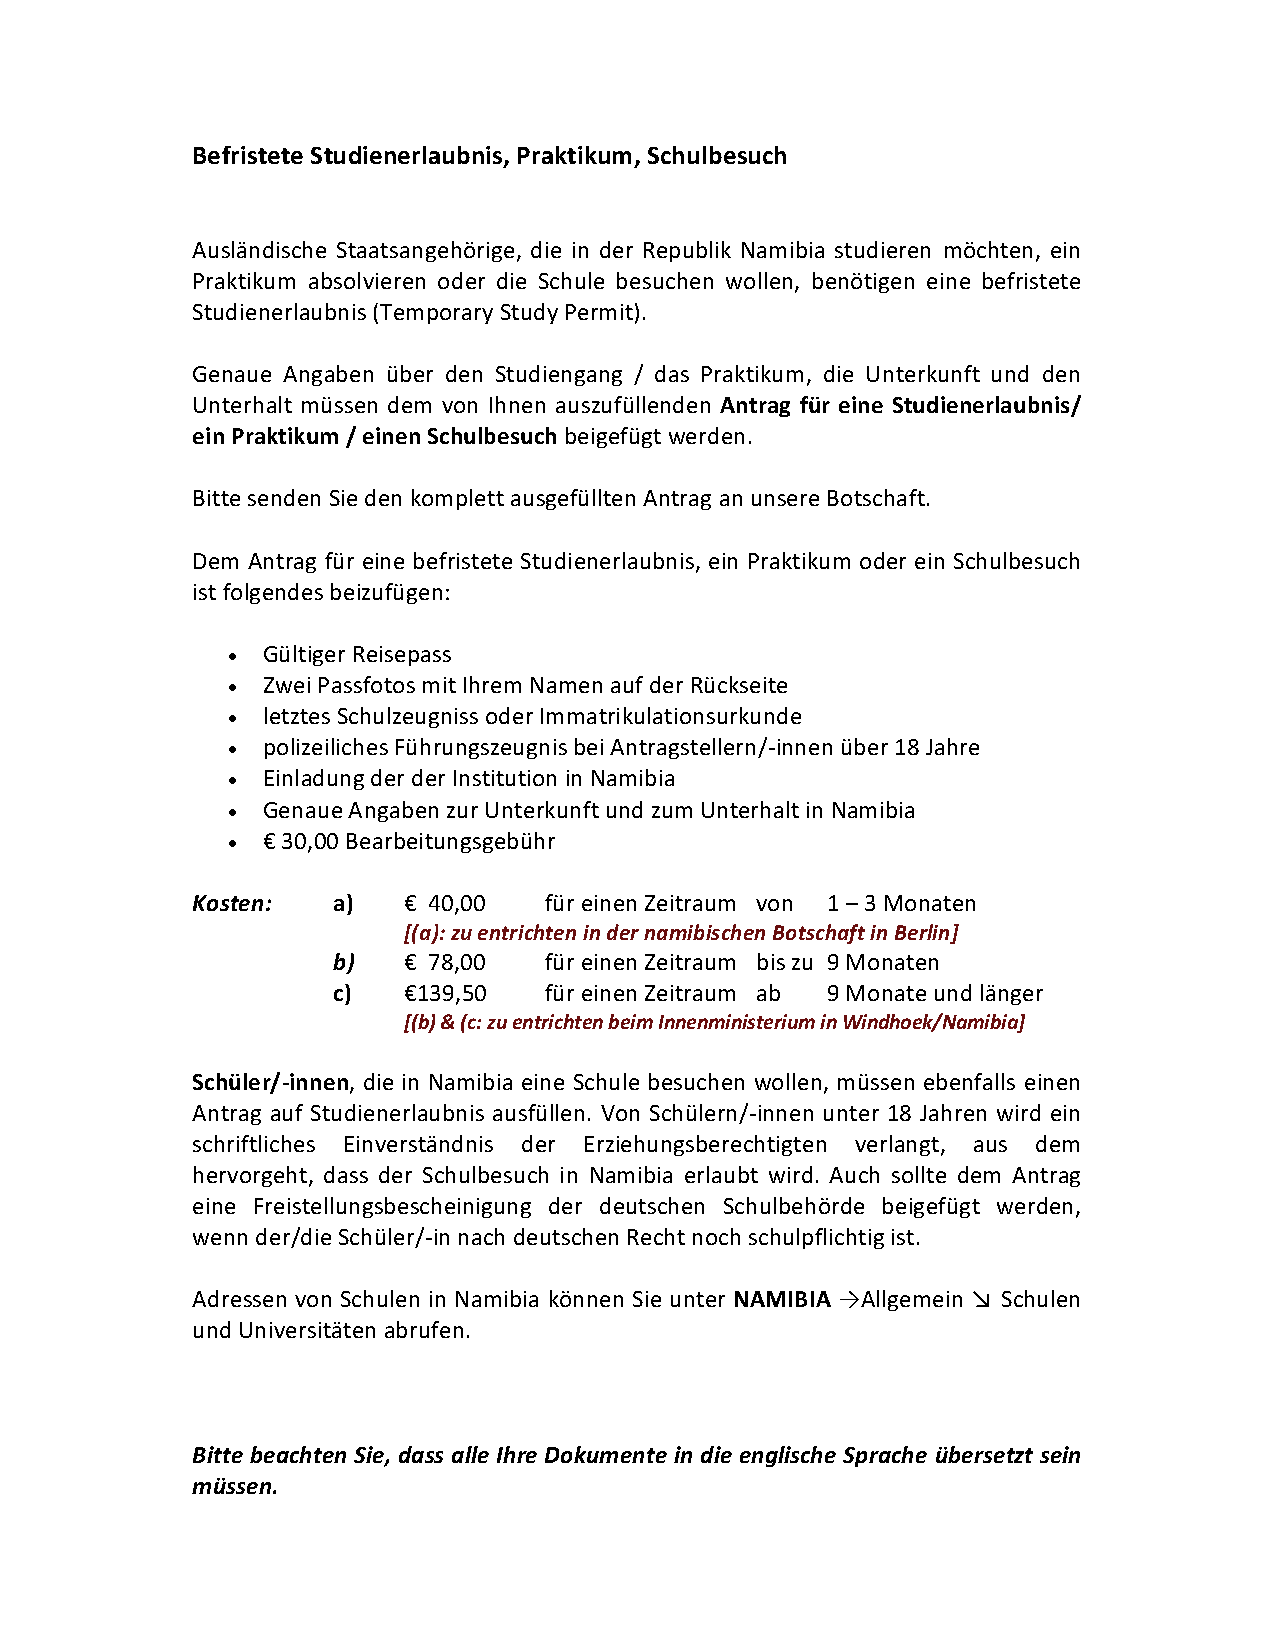
\includepdf[pagecommand={\thispagestyle{fancy}},noautoscale ,scale=0.9,pages=-]{merkblatt_befristete_studienerlaubnis.pdf}

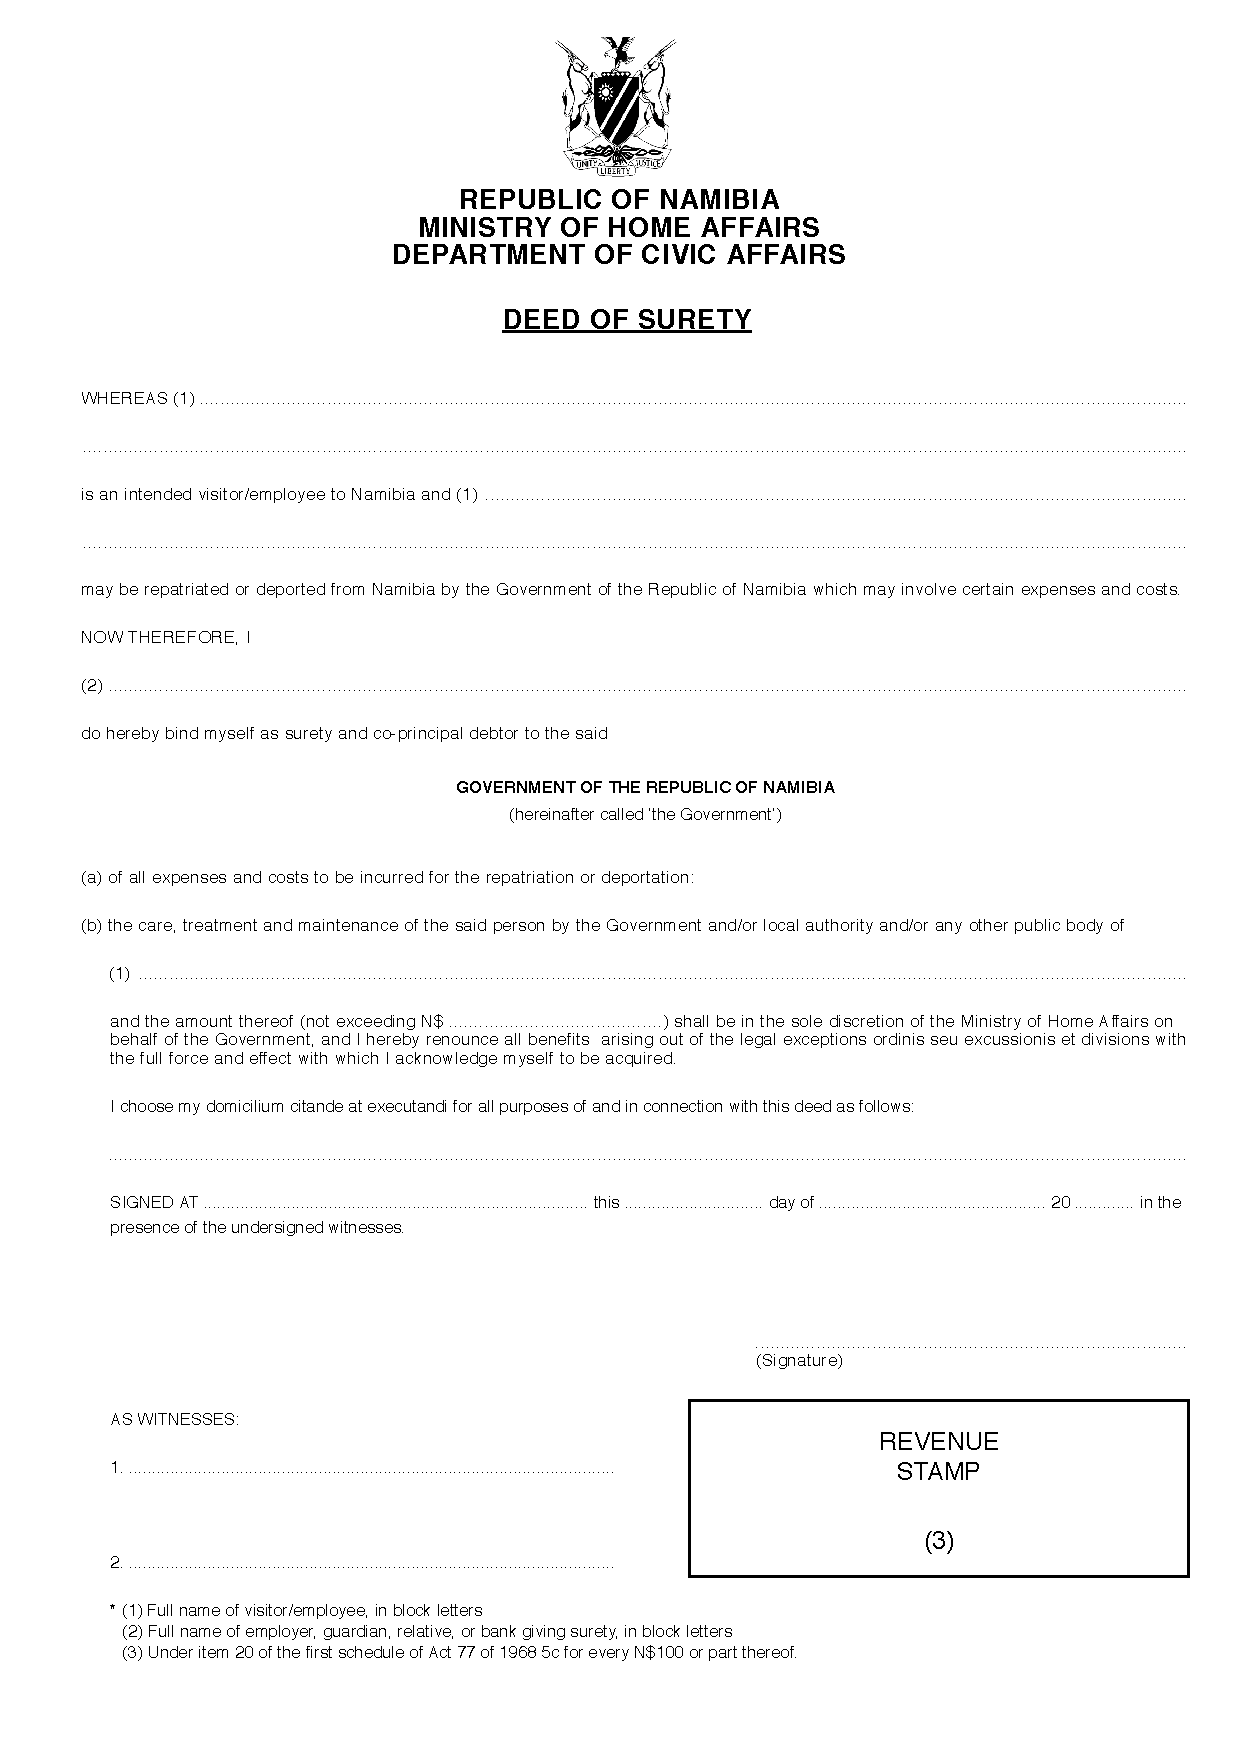
\includepdf[pagecommand={\thispagestyle{fancy}},noautoscale ,scale=0.9,pages=-]{Arbeitserlaubnis/deed_of_surety.pdf}

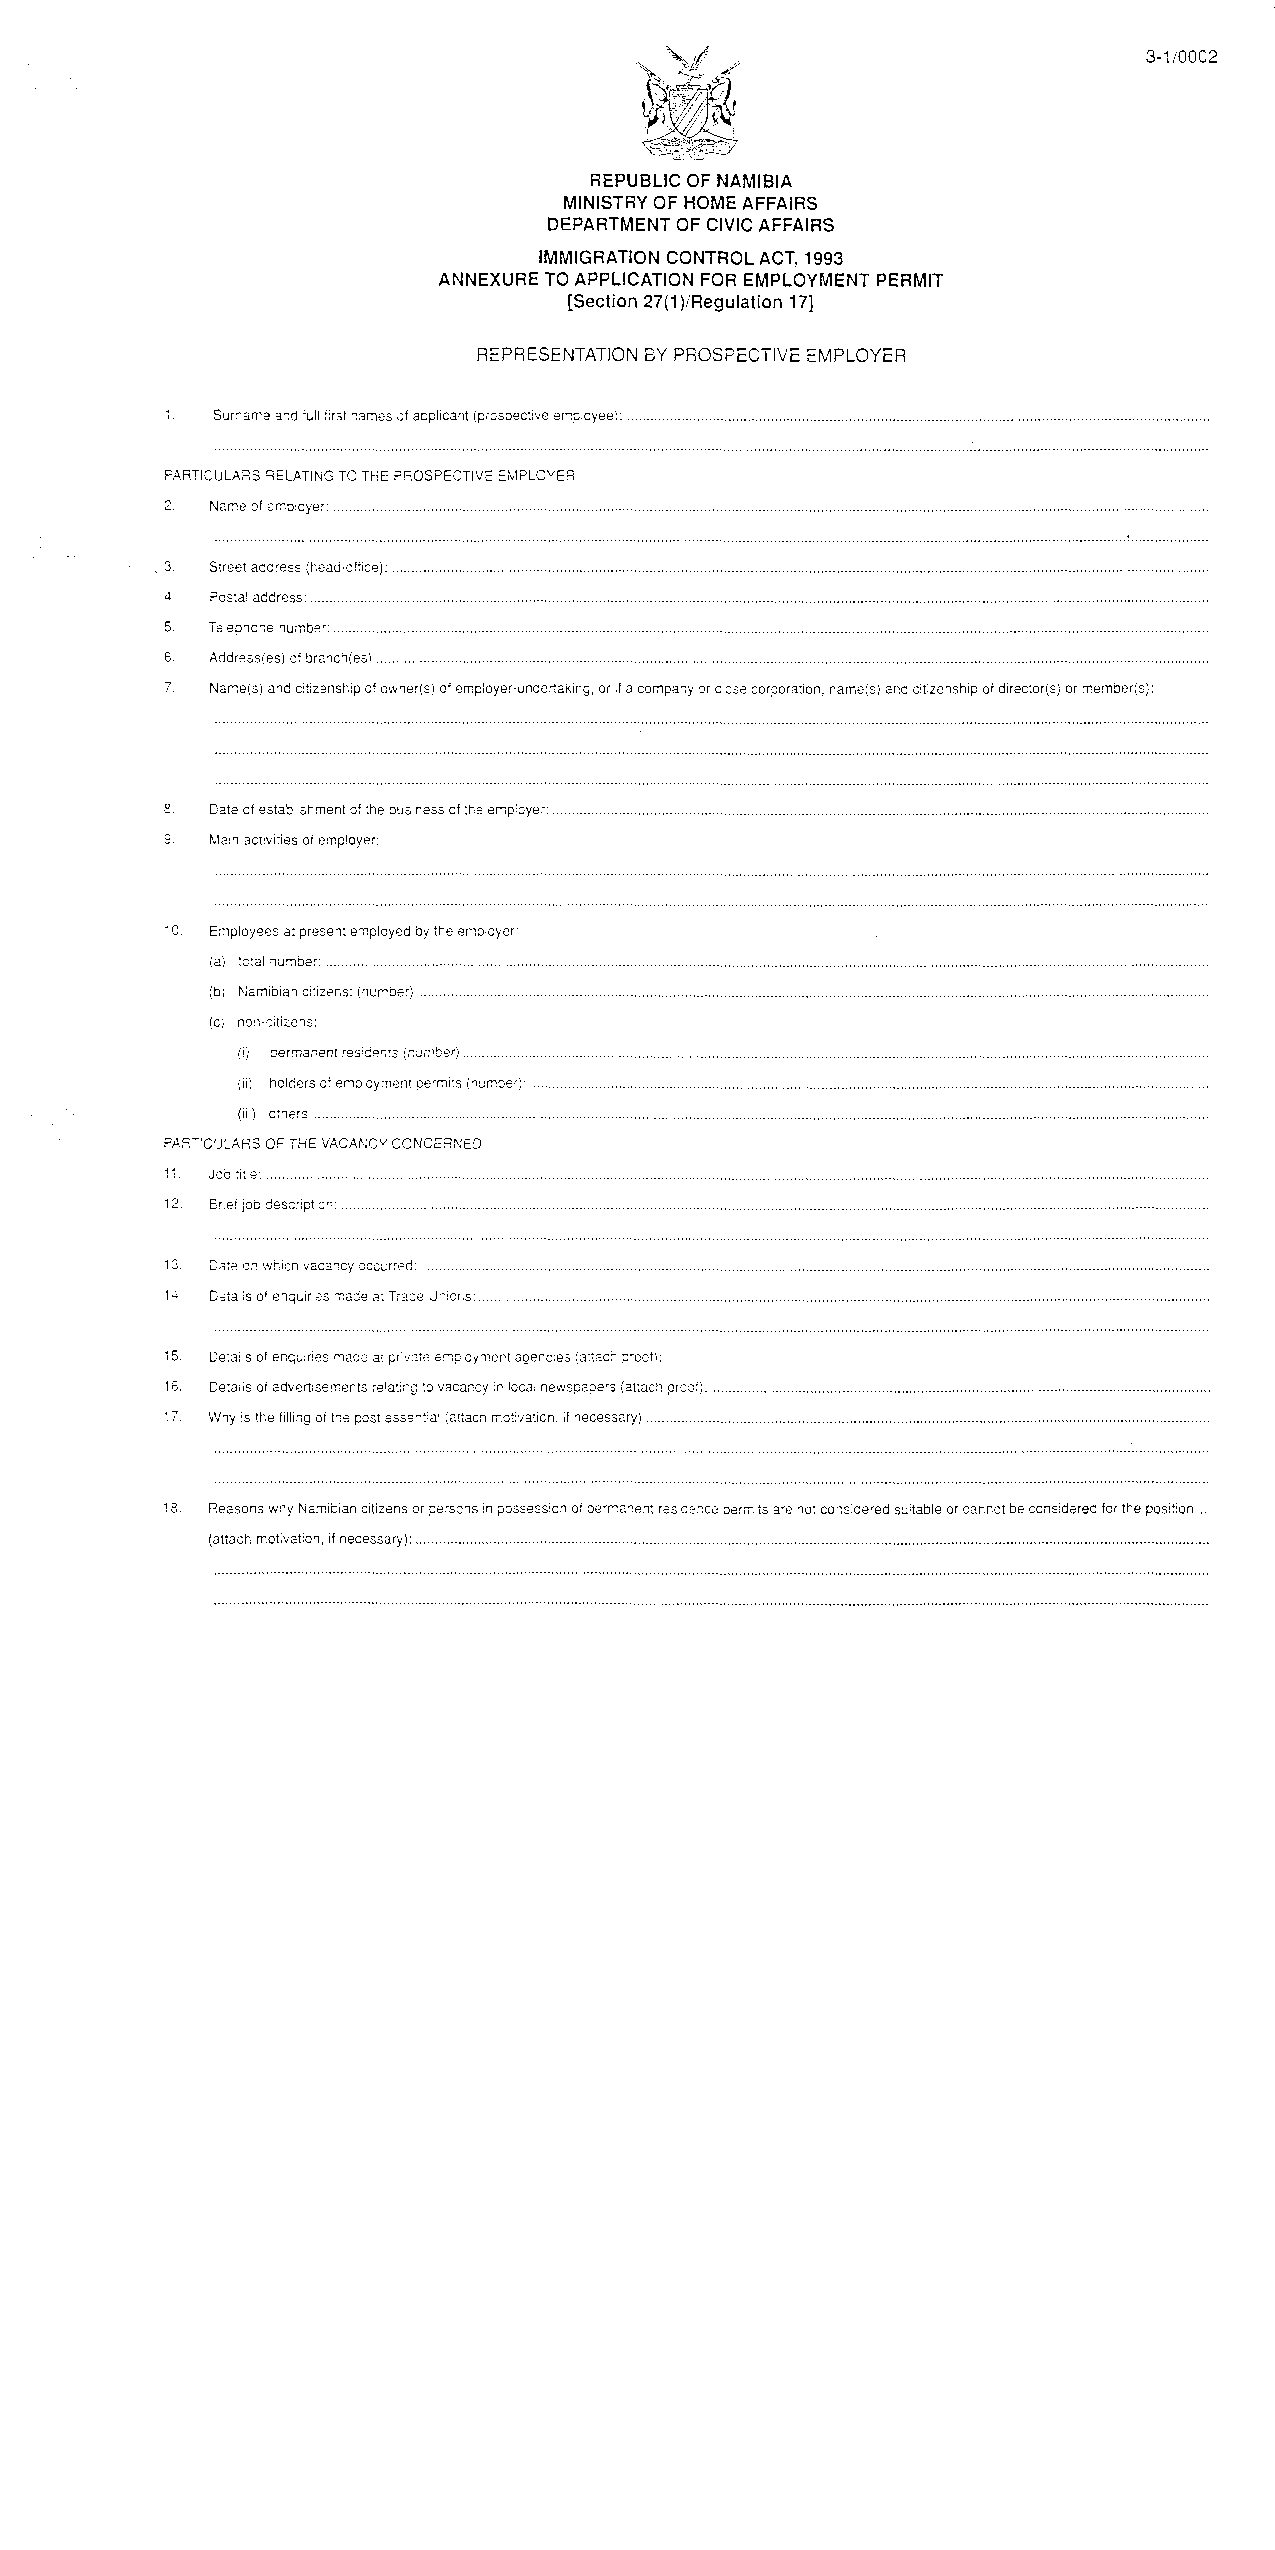
\includepdf[pagecommand={\thispagestyle{fancy}},noautoscale ,scale=0.9,pages=-]{Arbeitserlaubnis/prospective_employer_1.pdf}

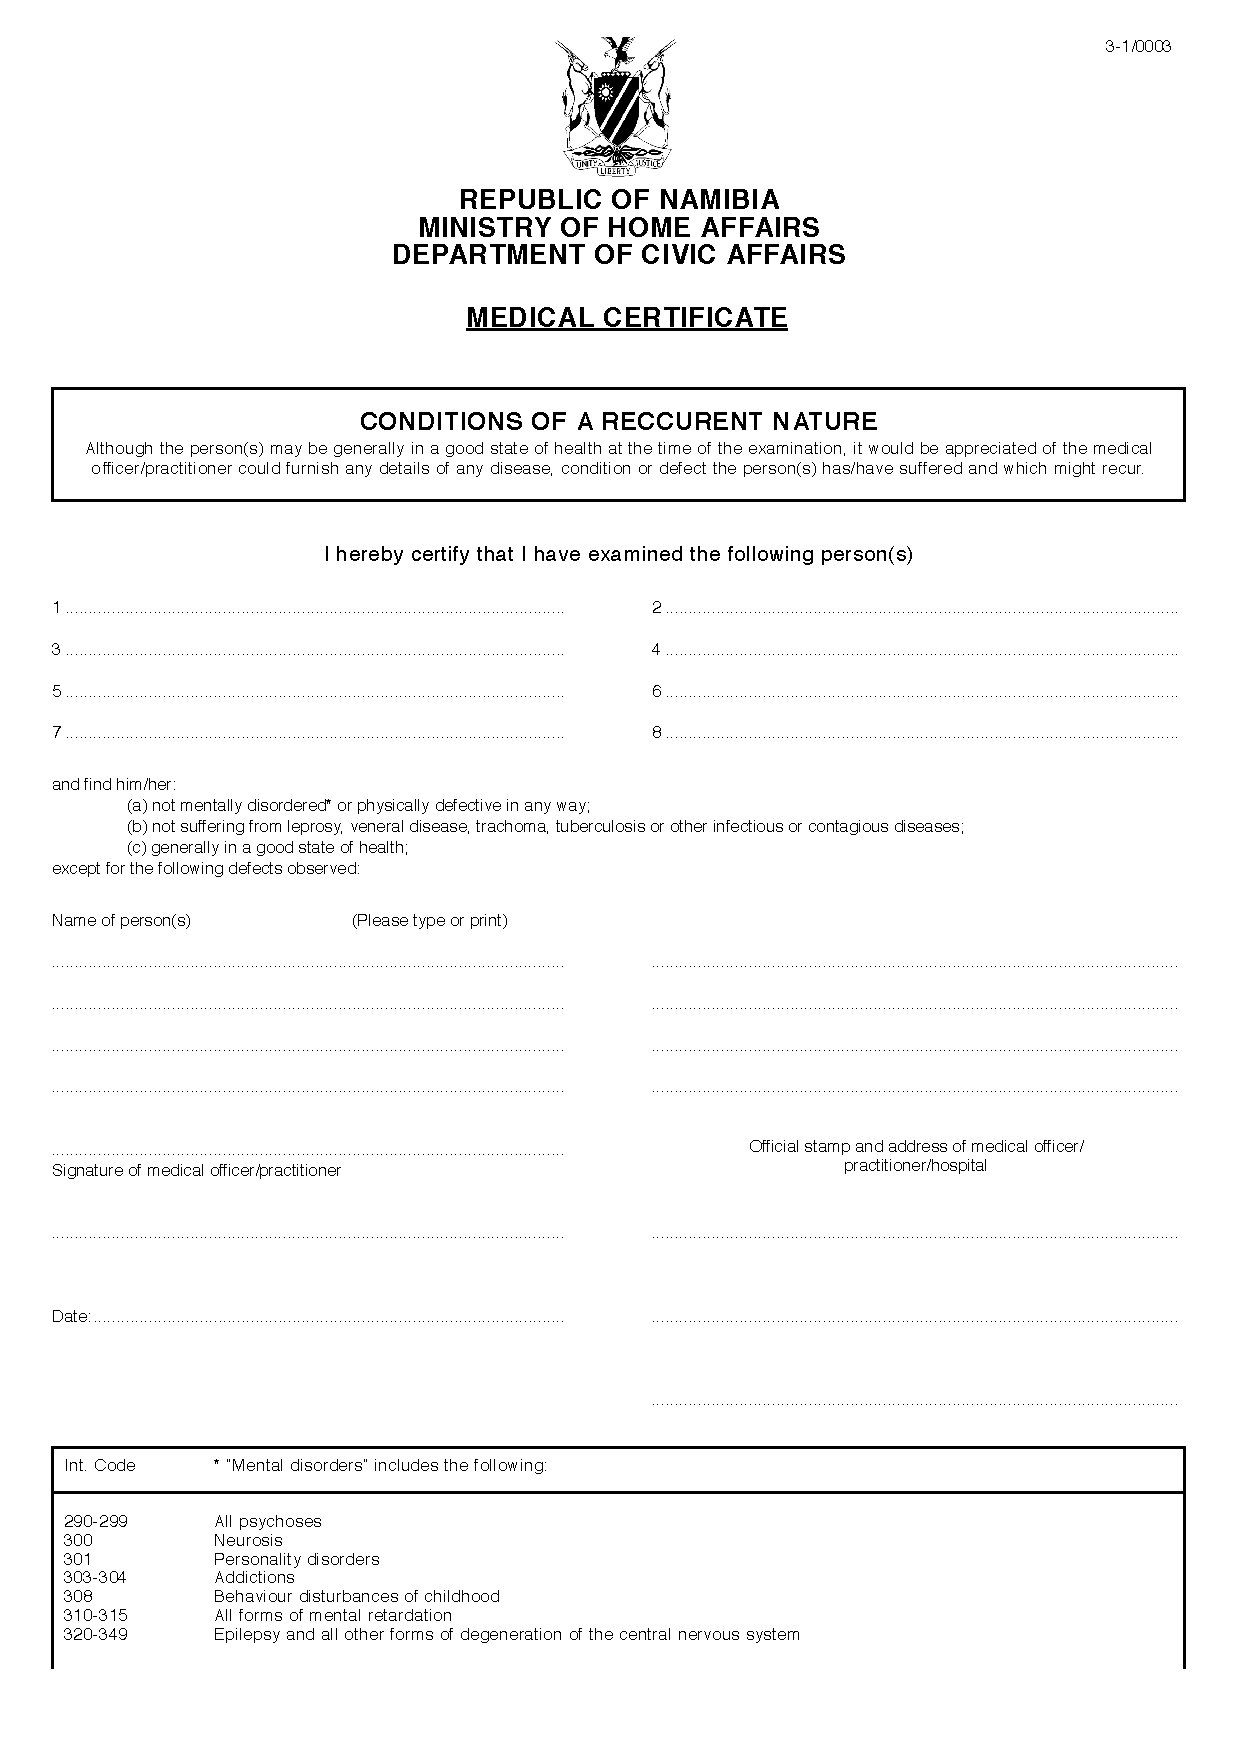
\includepdf[pagecommand={\thispagestyle{fancy}},noautoscale ,scale=0.9,pages=-]{Visum/Antrag_medical.pdf}

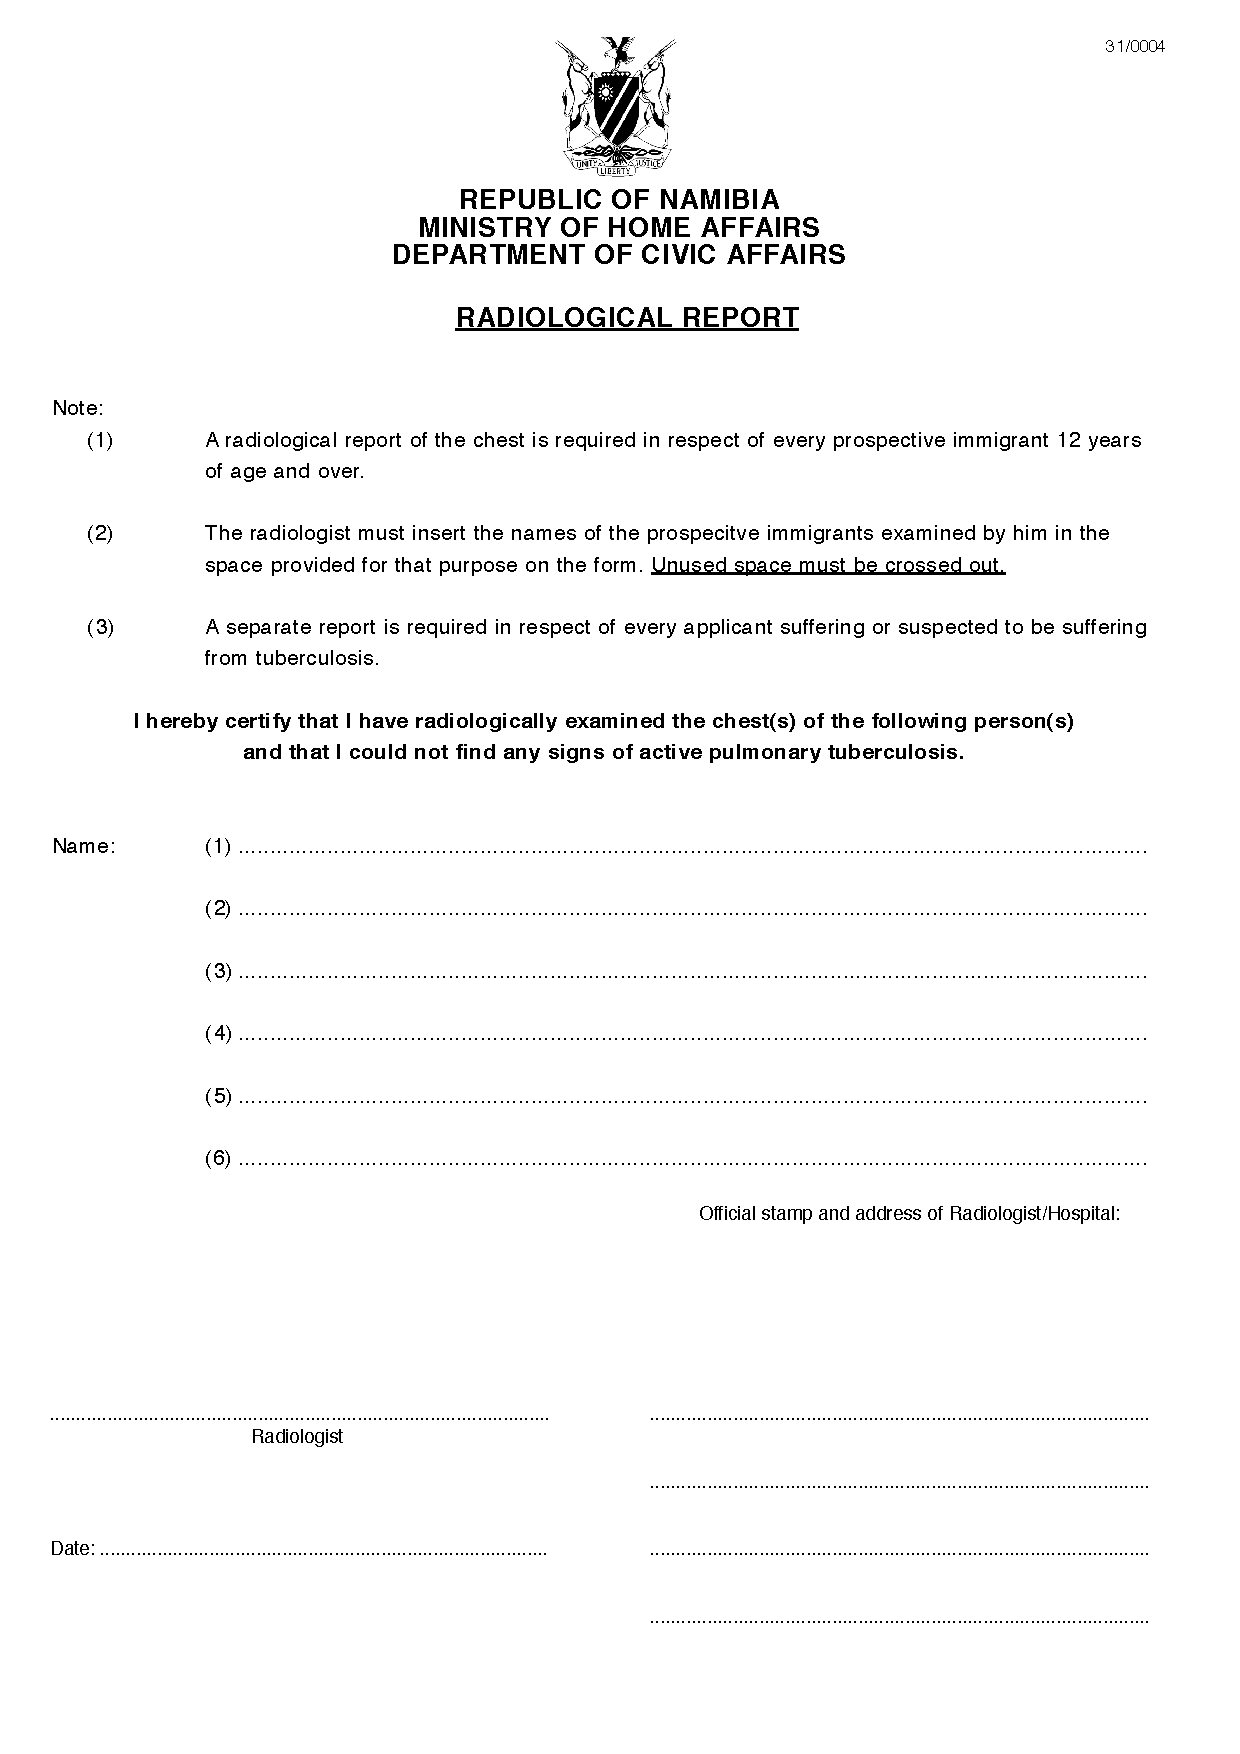
\includepdf[pagecommand={\thispagestyle{fancy}},noautoscale ,scale=0.9,pages=-]{Visum/Antrag_radiological.pdf}

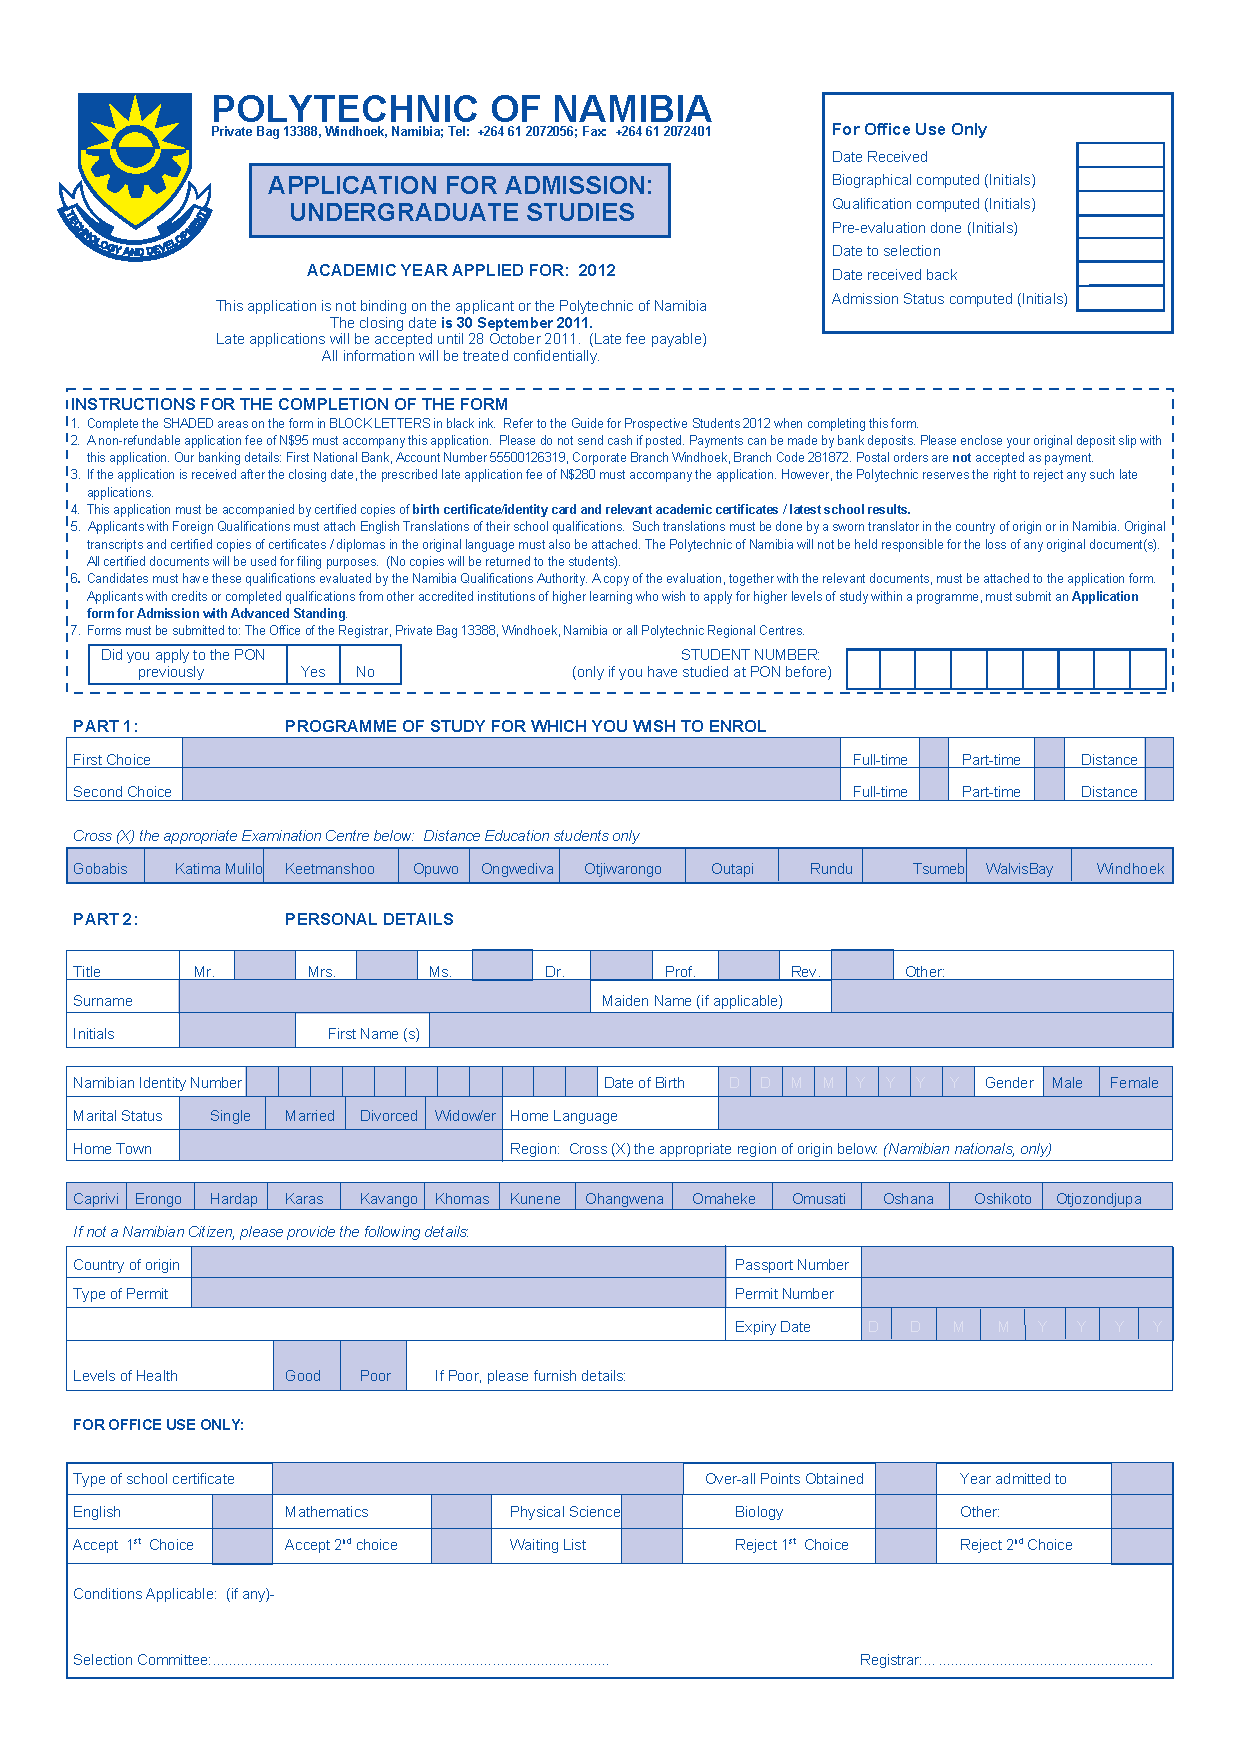
\includepdf[pagecommand={\thispagestyle{fancy}},noautoscale ,scale=0.9,pages=-]{Bewerbung_Schule/app_form.pdf}

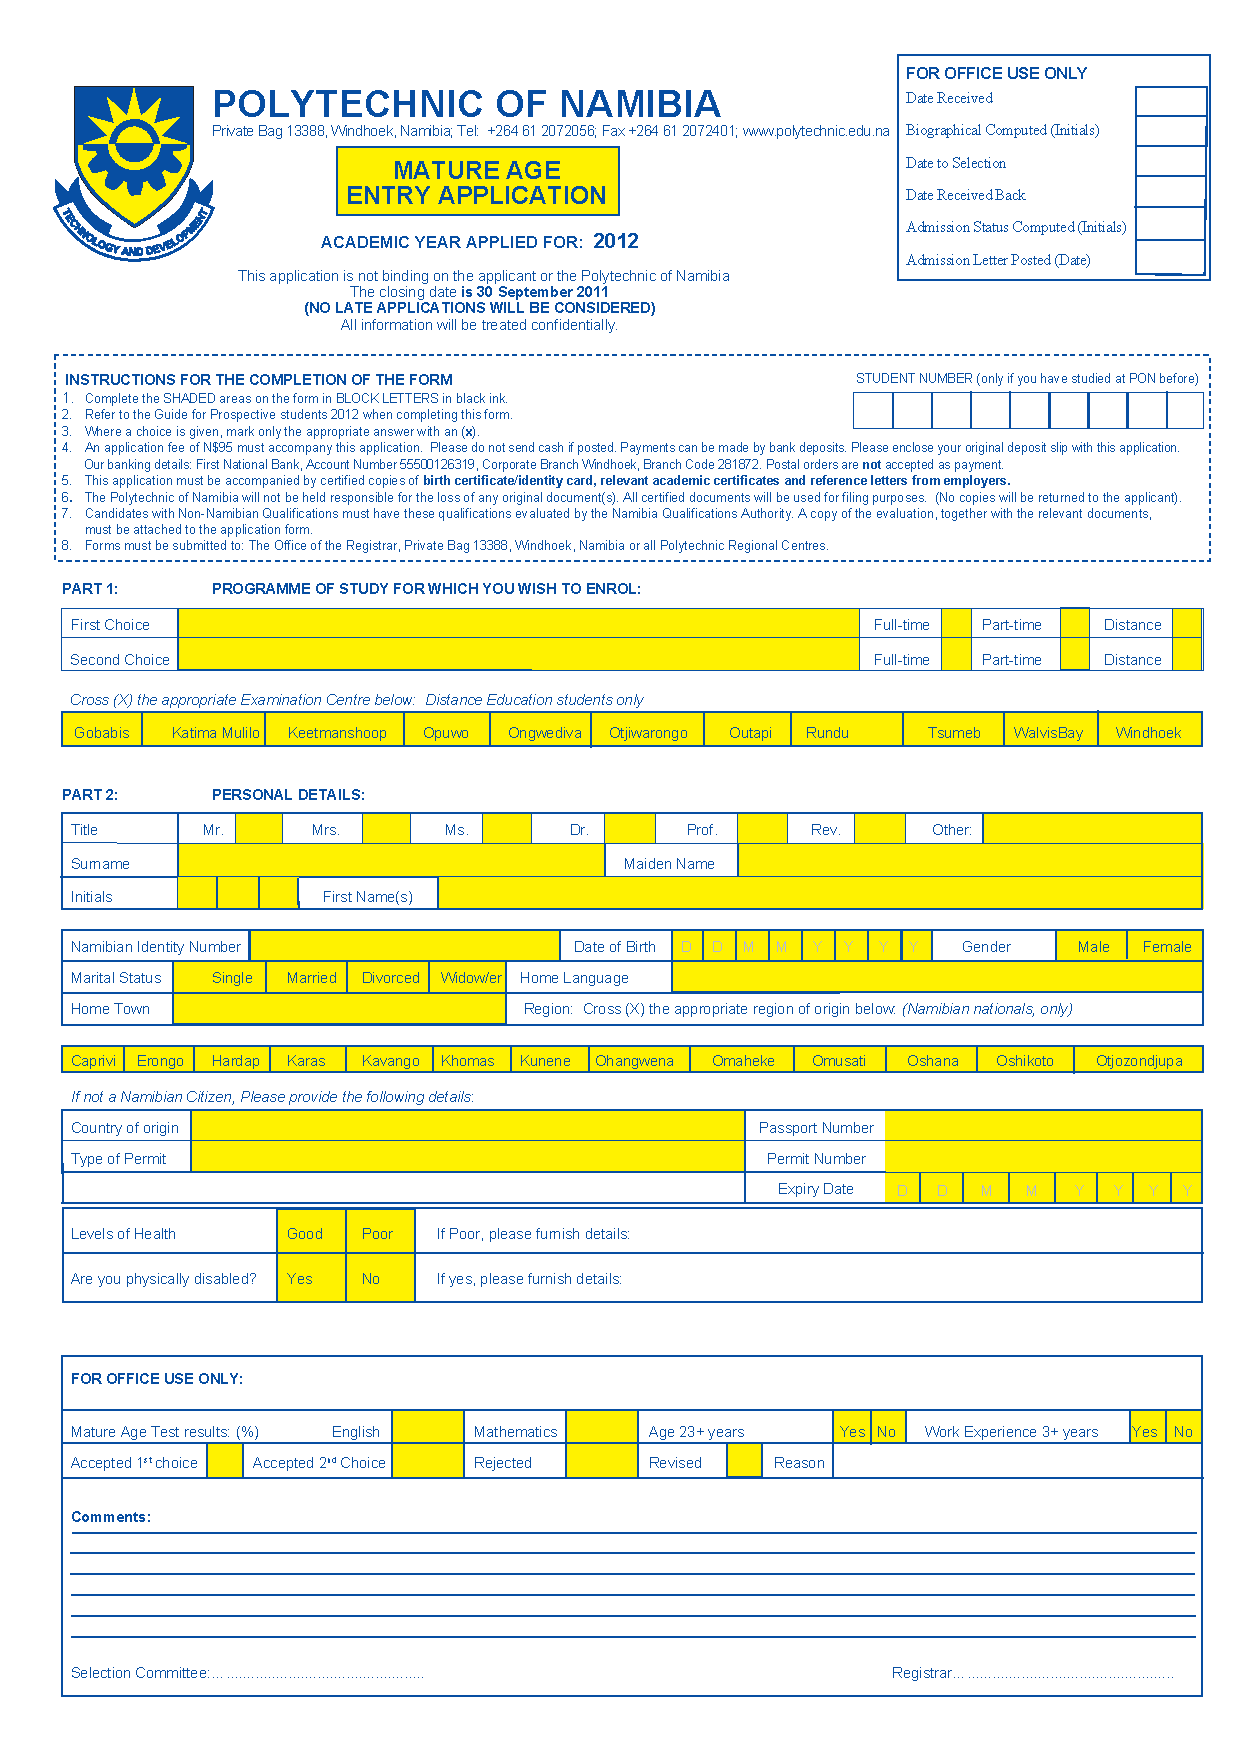
\includepdf[pagecommand={\thispagestyle{fancy}},noautoscale ,scale=0.9,pages=-]{Bewerbung_Schule/app_mature.pdf}

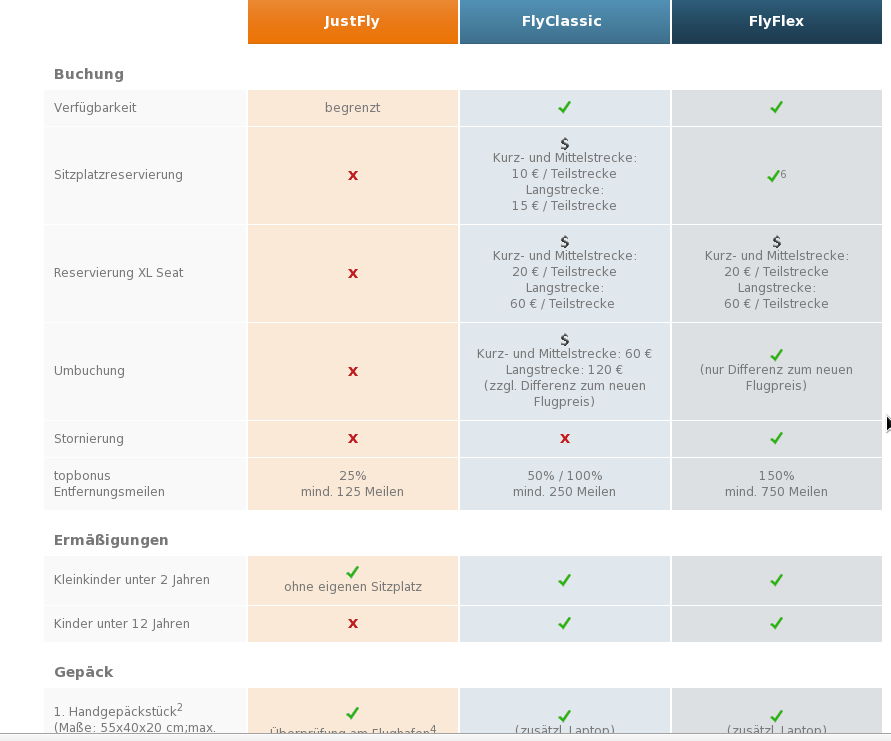
\includegraphics[scale=0.9]{Flug_Air_Berlin/Bildschirmfoto_am_2012-06-13_14_47_20.png} 

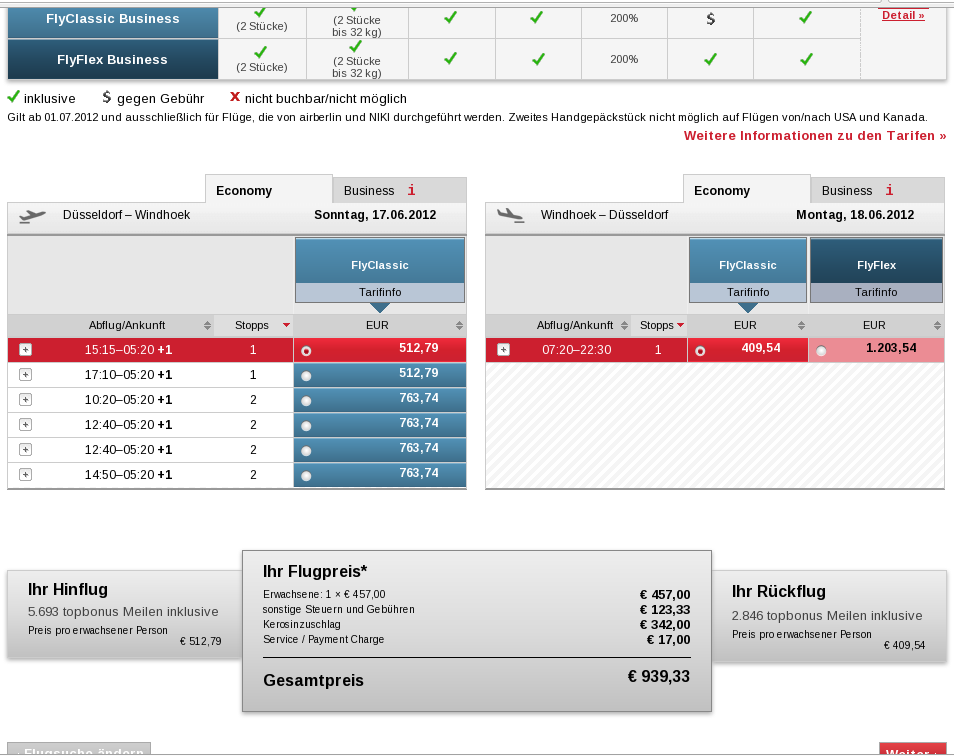
\includegraphics[scale=0.9]{Flug_Air_Berlin/Bildschirmfoto_am_2012-06-13_14_47_22.png} 

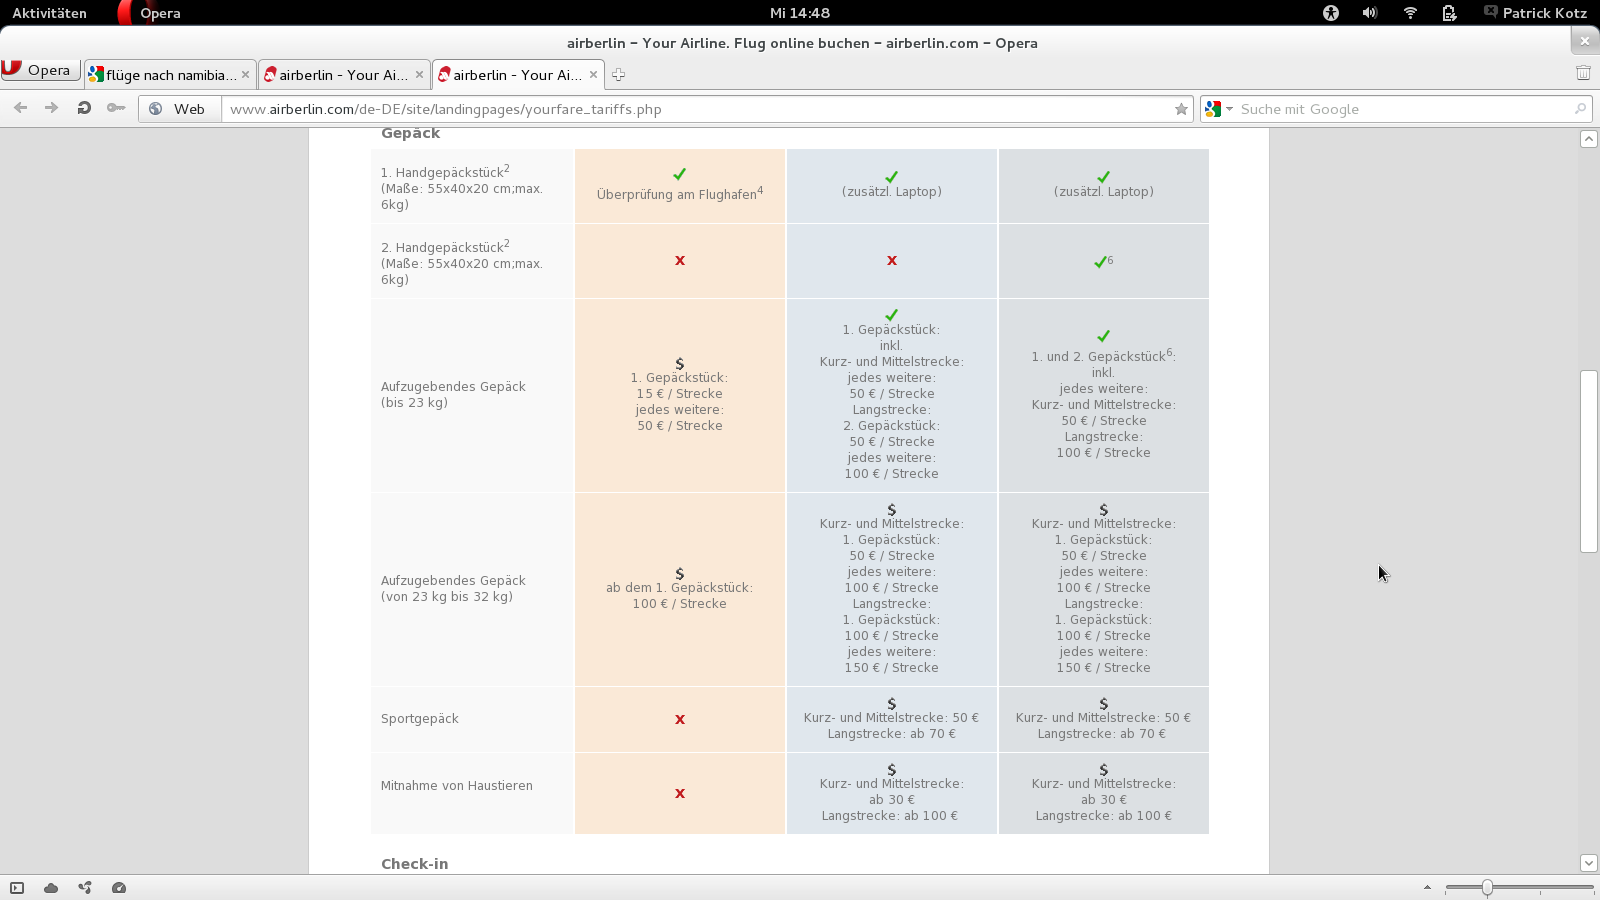
\includegraphics[scale=0.9]{Flug_Air_Berlin/Bildschirmfoto_am_2012-06-13_14_47_26.png} 

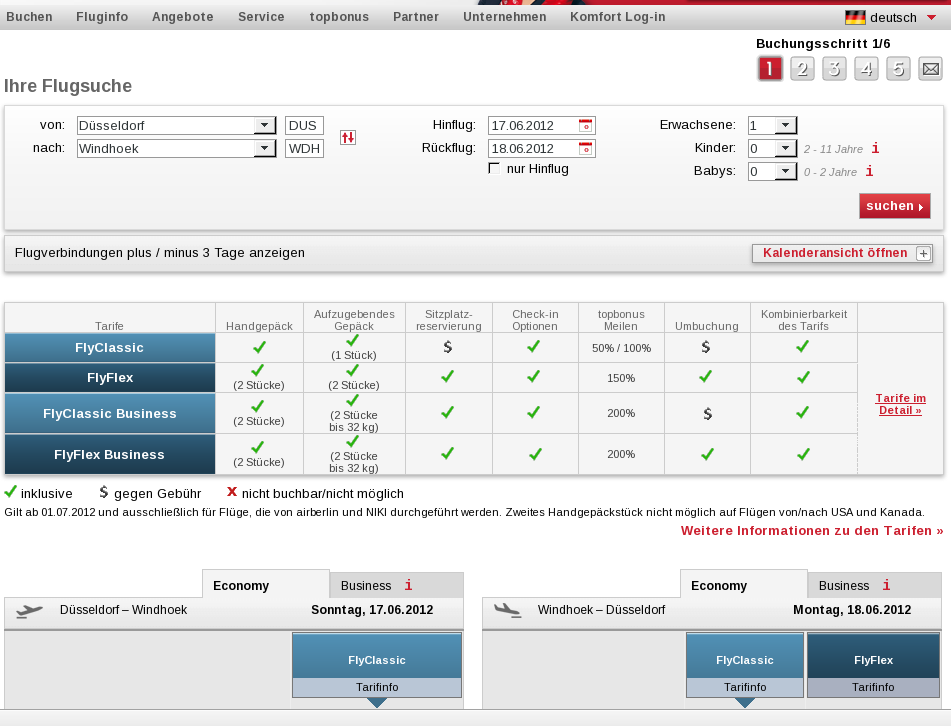
\includegraphics[scale=0.9]{Flug_Air_Berlin/Bildschirmfoto_am_2012-06-13_14_47_43.png} 

\end{document}
